% !TeX spellcheck = de_DE
\documentclass[a4paper, 12pt, twoside, openright
%, draft, showframe
]{memoir}
\usepackage[T1]{fontenc}
\usepackage[margin=2cm, bindingoffset=5mm, includeheadfoot]{geometry}
\usepackage[british, german]{babel}
\usepackage[hyperref=true]{acro}
\usepackage[backend=biber, style=ieee]{biblatex}
\usepackage{fancyhdr, graphicx, datetime2, fontspec, tikz, float, hologo, csquotes, tabulary, listings}
%\usepackage[protrusion=true,final]{microtype}
\usepackage{hyperref}
\usepackage[all]{hypcap}

\addbibresource{sources.bib}
\acsetup{
	first-style = short,
	list-style = longtable
}

\DeclareAcronym{dotnet}{
	short = .NET,
	long = .NET-Framework
}

\DeclareAcronym{rpi}{
	short = RPi,
	long = Raspberry Pi
}

\DeclareAcronym{rtsp}{
	short = RTSP,
	long = Real Time Streaming Protocol
}

\DeclareAcronym{sdk}{
	short = SDK,
	long = Software Development Kit
}

\DeclareAcronym{ndk}{
	short = NDK,
	long = Native Development Kit
}

\DeclareAcronym{fi}{
	short = FI,
	long = Fachspezifische Softwaretechnik
}

\DeclareAcronym{css}{
	short = CSS,
	long = Cascading Style Sheets
}

\DeclareAcronym{rtp}{
	short = RTP,
	long = Real-time Transport Protocol
}

\DeclareAcronym{rtcp}{
	short = RTCP,
	long = Real-Time Control Protocol
}

\DeclareAcronym{vod}{
	short = VOD,
	long = Video on Demand
}

\DeclareAcronym{apk}{
	short = APK,
	long = Android Package
}

\DeclareAcronym{eagle}{
	short = EAGLE,
	long = Easily Applicable Graphical Layout Editor
}

\DeclareAcronym{pcb}{
	short = PCB,
	long = Printed Circuit Board
}

\DeclareAcronym{smd}{
	short = SMD,
	long = Surface-mounted Device
}

\DeclareAcronym{ic}{
	short = IC,
	long = Integrated Circuit
}

\DeclareAcronym{uwp}{
	short = UWP,
	long = Universal Windows Platform
}

\DeclareAcronym{tht}{
	short = THT,
	long = Through-Hole Technology
}

\DeclareAcronym{clr}{
	short = CLR,
	long = Common Language Runtime
}

\DeclareAcronym{cil}{
	short = CIL,
	long = Common Interface Language
}

\DeclareAcronym{mvvm}{
	short = MVVM,
	long = Model-view-viewmodel
}

\DeclareAcronym{cpu}{
	short = CPU,
	long = Central processing unit
}

\DeclareAcronym{ietf}{
	short = IETF,
	long = Internet Engineering Task Force
}

\DeclareAcronym{http}{
	short = HTTP,
	long = Hypertext Transfer Protocol
}

\DeclareAcronym{url}{
	short = URL,
	long = Uniform Resource Locator
}

\DeclareAcronym{ui}{
	short = UI,
	long = User interface
}

\DeclareAcronym{xaml}{
	short = XAML,
	long = Extensible Application Markup Language
}

\DeclareAcronym{xml}{
	short = XML,
	long = Extensible Markup Language
}

\DeclareAcronym{wysiwym}{
	short = WYSIWYM,
	long = What You See Is What You Mean
}

\emergencystretch=1em

\hypersetup{
	linktoc=all,
	colorlinks=false,
	linkcolor=blue
}

% pagestyles ------------------------------------------------------------------
\fancypagestyle{normalpage}{
	\fancyhf{} %clear header and footer
	\rhead[\leftmark]{\thepage}
	\lhead[\thepage]{\rightmark}
	\cfoot{\authorName}
	\renewcommand{\headrulewidth}{0.4pt}
	\renewcommand{\footrulewidth}{0.4pt}
}
\aliaspagestyle{chapter}{normalpage}

\fancypagestyle{abstractpage}{
	\fancyhf{} %clear header and footer
	\rhead[]{\thepage}
	\lhead[\thepage]{}
	\cfoot{\authorName}
	\renewcommand{\headrulewidth}{0.4pt}
	\renewcommand{\footrulewidth}{0.4pt}
}
\aliaspagestyle{part}{abstractpage}

\fancypagestyle{titlepage}{
	\fancyhf{} %clear header and footer
	\fancyhead[c]{
\includegraphics[width=\linewidth]{images/HTL_Header}}
	\cfoot{\authorName}
	\renewcommand{\headrulewidth}{0.4pt}
	\renewcommand{\footrulewidth}{0.4pt}
}
\aliaspagestyle{titlingpage}{titlepage}

% memoir configuration ------------------------------------------------------
\chapterstyle{section}
\setsecnumdepth{subsection}
\settocdepth{subsection}

% custom commands -----------------------------------------------------------
\newcommand{\blankpage}{
	\newpage
	\null
	\thispagestyle{empty}
	\newpage
}
\newcommand{\MarioPrantl}{DI(FH) Mario Prantl}
\newcommand{\AndreasGrain}{Andreas Grain}
\newcommand{\MatthiasMair}{Matthias Mair}
\newcommand{\authorName}{\AndreasGrain / \MatthiasMair}
\newcommand{\crossref}[1]{\emph{\ref{#1} \nameref{#1}}}

% text formatting ----------------------------------------------------------
%\setlength{\parindent}{0pt}% Remove paragraph indentation
\setlength{\parskip}{8pt}% Add space after paragraph
\setmainfont{Arial}
\renewcommand{\footnotesize}{\scriptsize}
\lstset{basicstyle=\ttfamily\small,breaklines=true}

% Document start -----------------------------------------------------------
\begin{document}
\pagestyle{normalpage}

\frontmatter
\begin{titlingpage}
	\newgeometry{margin=2cm, bindingoffset=5mm, includeheadfoot, headheight=54pt}
\begin{center}
	\vspace*{2cm}
	\Huge\textbf{Diplomarbeit}\\
	\vspace*{2cm}
	\huge Bidirektionale Videosprechanlage\\
	\vspace*{0.5cm}
	\normalsize Erweiterung einer RaspberryPi basierten Videogegensprechanlage\\
	\vspace*{1.5cm}
	\textbf{Höhere Technische Bundeslehr- und Versuchsanstalt Anichstraße}\\
	\vspace*{0.5cm}
	\rule{0.75\linewidth}{0.4pt}\\
	\vspace*{0.5cm}
	Abteilung Elektrotechnik\\
	\vspace*{1cm}
	\begin{minipage}{0.425\linewidth}
		\begin{flushleft}
			Ausgeführt im Schuljahr 2019/20 von:\bigskip\\
			Andreas Grain 5AHET (HV)\\
			Matthias Mair 5AHET\\
		\end{flushleft}
	\end{minipage}
	\begin{minipage}{0.425\linewidth}
		\begin{flushright}
			Betreuer:\bigskip\\
			DI(FH) Mario Prantl\\
		\end{flushright}
	\end{minipage}
\end{center}
\vspace*{1cm}
%\hspace*{0.15\linewidth}Projektpartner: keine
\vfill
Innsbruck, am \today
\vspace*{1cm}
\hrule
\vspace*{1cm}
\noindent\begin{minipage}{0.495\linewidth}
	Abgabevermerk:	
\end{minipage}
\noindent\begin{minipage}{0.495\linewidth}
	Betreuer:	
\end{minipage}
\begin{flushleft}
	Datum:
\end{flushleft}
\restoregeometry
\end{titlingpage}

\OnehalfSpacing

\chapter{Erklärungen}
\section{Eidesstattliche Erklärung}
Wir erklären an Eides statt, dass wir die vorliegende Diplomarbeit selbständig und ohne fremde Hilfe verfasst, andere als die angegebenen Quellen und Hilfsmittel nicht benutzt und die den benutzten Quellen wörtlich und inhaltlich entnommenen Stellen als solche erkenntlich gemacht haben.
\vspace*{1.5cm}
\begin{center}
	\hrule
	\vspace*{0.2cm}
	Ort, Datum\hspace*{0.4\linewidth}\AndreasGrain\\
	\vspace*{1.5cm}
	\hrule
	\vspace*{0.2cm}
	Ort, Datum\hspace*{0.4\linewidth}\MatthiasMair
\end{center}
\vspace*{1.5cm}

\section{Gender-Erklärung}
Aus Gründen der besseren Lesbarkeit wird in dieser Diplomarbeit die Sprachform des generischen Maskulinums angewendet.
Es wird an dieser Stelle darauf hingewiesen, dass die ausschließliche Verwendung der männlichen Form geschlechtsunabhängig verstanden werden soll.
\cleartoverso

\tableofcontents
%\cleartoverso

\chapter{Kurzfassung/Abstract}
\section{Deutsch}
Die vorliegende Diplomarbeit beschäftigt sich mit der Erweiterung einer \ac{rpi}-basierten Videosprechanlage um eine Smartphone-Applikation, sowie der grundlegenden Überarbeitung der Stations-Hardware.
Zusätzlich soll ein Linux-basierter, aus dem Internet erreichbarer Server zum Verteilen der Video-Streams eingerichtet werden.
%Für die Entwicklung der Smartphone-App wird das Xamarin-Framework herangezogen, sodass die Applikation sowohl auf Android-, als auch iOS-Geräten lauffähig ist.
\par
Dieses Projekt basiert auf einer früheren Diplomarbeit von Sebastian Wagner und Tobias Pfluger an der HTL Anichstraße aus dem Jahr 2017/18, welche ein voll funktionsfähiges Videosprechanlagensystem hervorbrachte.
Jedoch wurde damals die Hardware-Entwicklung sehr vernachlässigt.
\par
Die Hardware-Erweiterung besteht grundsätzlich aus zwei Teilen: zum einen werden die vielen Elektronik-Bausteine in einer zentralen Platine vereint, was eine einfachere und kostengünstigere Fertigung erlaubt.
Zusätzlich wird die aktuelle Hardware der Station um einen Watchdog-Timer erweitert, welcher im Fehlerfall die Anlage zurücksetzt.
\par
Softwareseitig wird die Anlage um eine Smartphone-App ausgebaut, mit welcher der Fernzugriff auf das System ermöglicht werden soll.
\par
\newpage

\begin{otherlanguage}{british}
	\section{English}
	This diploma thesis deals with the extension of a \ac{rpi}-based video intercom system by a smartphone application, as well as the fundamental revision of the station hardware.
	In addition, a Linux-based server, accessible from the Internet, will be set up to distribute the video streams.
	%The Xamarin framework will be used for the development of the smartphone app, so that the application can be run on both Android and iOS devices.
	\par
	This project is based on an earlier diploma thesis by Sebastian Wagner and Tobias Pfluger at the HTL Anichstraße from the year 2017/18, which produced a fully functional video intercom system.
	However, at that time the hardware development was rather neglected.
	\par
	The hardware extension basically consists of two parts: on the one hand, the many electronic components are combined in a central circuit board, which allows easier and more cost-effective production.
	In addition, the current hardware of the station is extended by a watchdog timer, which resets the system in case of an error.
	\par
	On the software side, the system will be extended by a smartphone app, which will enable remote access to the system.
	\par
\end{otherlanguage}
\chapter{Projektergebnis} 
%\thispagestyle{abstractpage}
%iOS-Entwicklung nicht durchgeführt, kein Mac vorhanden.
%Mehrfachzugriff über App wurde nicht eingeschränkt, ist weiter zu bearbeiten.

\mainmatter
\chapter{Einleitung}
Jedes moderne Wohngebäude ist inzwischen mit einer Gegensprechanlage ausgestattet.
Eine solche Anlage erlaubt es dem Wohnungsbesitzer mit jemandem vor der Haustür zu kommunizieren, bevor dieser hereingelassen wird.
Manche Wohnungen besitzen bereits eine Videosprechanlage, die dem Bewohner nicht nur den Ton, sondern zusätzlich ein Video von der Außenstelle bereitstellt.
Dem Gast wird jedoch immer noch nur der Ton von innen übertragen.
Diese Applikation ist ortsgebunden, d.h. es müssen sowohl der Gast, als auch der Bewohner vor der entsprechenden Station stehen.\par

Im Zuge einer früheren Diplomarbeit des Schuljahres 2017/18 an der HTL Anichstraße entwickelten Sebastian Wagner und Tobias Pfluger eine Videogegensprechanlage, welche mehrere Innenstationen und die bidirektionale Video- und Tonübertragung unterstützt.
Die Idee ist, dass in einem Wohnungskomplex pro Partei eine Innenstation verbaut wird, sowie eine Außenstation am Hauseingang.
Die einzelnen Innenstationen, also Wohnungsparteien, können dann nicht nur mit der Außenstation, sondern auch mit anderen Innenstationen per Video und Ton kommunizieren.
Die Stationen wurden mit Hilfe eines \ac{rpi} realisiert, um die Kosten gering zu halten.\par

Am Anfang des 5. Schuljahres im Herbst 2019 wurde uns von unserem FI-Professor \MarioPrantl\ angeboten, dieses Projekt durch eine Smartphone-App und eine Hardware-Überarbeitung zu verbessern.
Für die Entwicklung der App sollte das Xamarin-Rahmenwerk verwendet werden, damit die Applikation auf sowohl Android- als auch iOS-Geräten lauffähig ist. 
Der Benutzer soll über die App das Video der entsprechenden Station abrufen und mit dem Gesprächspartner sprechen können.
Hierfür wird ein aus dem Internet erreichbarer Medien-Verwaltungsserver benötigt, der die Medien-Streams der Einzelstationen empfängt und an die Station des Gesprächspartners überträgt.
Die Hardware-Überarbeitung hat mehrere Ziele; zum einen soll dadurch die Komplexität des internen Aufbaus einer Station verringert werden.
Zum anderen soll mit Hilfe eines Watchdog-Timers das Langzeit-Betriebsverhalten verbessert werden.

\section{Funktionalität}
\paragraph{Ortsunabhängiger Anlagenzugriff:}
Um dem Anwender mehr Komfort bieten zu können, beschränkt sich die Anlage und dessen Funktion nicht mehr auf die fest installierte Station, sondern ist auch über ein mobiles Gerät bedienbar.
Dies bietet den Vorteil, dass auch wenn man sich gerade nicht in der Nähe der Innenstation befindet, mit Besuchern kommuniziert werden kann.

\paragraph{Paketdienst:}
Die Paketübergabe erfolgt üblicherweise persönlich.
Wenn der Empfänger nicht zuhause ist, nimmt der Paketzusteller die Ware wieder mit, deponiert sie bei einer Paketabholstelle und hinterlässt dem Empfänger lediglich eine Benachrichtigung.
Diese Vorgangsweise ist besonders ärgerlich, wenn man den Paketzusteller um wenige Minuten versäumt hat oder nicht schnell genug zur Innenstelle gelangen konnte.
Beispielsweise befindet sich der Bewohner gerade auf dem Dachboden oder im Keller.
Mit einer Smartphone-App ist eine sofortige Kontaktaufnahme mit dem Paketzusteller möglich und verhindert eine unnötige zusätzliche Bearbeitung des Paketversandes.

\paragraph{Sicherheit:}
Die neu gewonnene Ortsunabhängigkeit der Anlage bietet eine höhere Einbruchssicherheit, da man jederzeit Überblick über erwünschte bzw. unerwünschte Besucher hat.
Über die Smartphone-Applikation ist das Öffnen des Türschlosses aus mehreren Gründen nicht möglich:
\begin{itemize}
    \item Wenn der Benutzer nicht zuhause ist, ist eine Türöffnung in den allermeisten Fällen nicht erwünscht.
    \item Wenn der Benutzer zuhause ist, muss er sowieso zur Eingangstür gehen, um den Besuch in Empfang zu nehmen. Die im Eingangsbereich installierte Station dient hier zur Öffnung der Haustür.
    \item Falls unbefugter Zugriff auf die Applikation erfolgen sollte, besteht kein besonderes Sicherheitsrisiko hinsichtlich Einbruchs in die Wohnung.
\end{itemize}

\section{Aufgabenteilung}
\paragraph{Andreas Grain} ist der Projekt-Hauptverantwortliche und zuständig für die App-Pro\-gram\-mierung.
Dies beinhaltet die Einarbeitung in und Verwendung des Xamarin-Rahmenwerks zur Erstellung einer Multiplattform-Smartphone-Applikation.
Diese soll den Video-Stream der gewählten Station abrufen und anzeigen, sowie den Mikrofon-Ton des Mobilgerätes zur Anlage zurückschicken.
Weiters ist er für die Einarbeitung in das GStreamer-Rahmenwerk zur zentralen Verarbeitung der Video- und Audio-Daten der Stationen und Mobilgeräte über einen Linux-basierten Server zuständig.
Darüber hinaus organisiert Andreas Grain sämtliche Treffen mit dem Betreuer, achtet auf die Einhaltung des Zeitplans und ist zuständig für das Erstellen des \hologo{XeLaTeX}-Dokuments

\paragraph{Matthias Mair} ist verantwortlich für die Hardware-Überarbeitung der Station.
Diese beinhaltet die Einarbeitung in das \ac{pcb}-Entwicklungsprogramm \ac{eagle} von der Firma Autodesk mit der Version 9.5.2, sowie das Recherchieren und Auswählen möglicher Verstärker-Schaltungen und -\acp{ic} für die Mikrofon- und Lautsprecher-Verstär\-kung.
Im Zuge der Hardware-Überarbeitung sollen die vielen Einzelmodule in einer übersichtlichen Platine vereint werden.
Für die Leiterplatte soll die weit verbreitete \ac{smd}-Technologie verwendet werden, da diese heutzutage Marktstandard für integrierte Geräte ist und im Vergleich zu traditionellen \ac{tht}-Platinen viel platzsparender ist.
Zusätzlich wird die Station um einen Watchdog-Timer erweitert, den Matthias Mair entwirft und die dazugehörige Software schreibt.

\section{Hinweise und Definitionen}
In diesem Dokument werden technische Begriffe aus der Elektronik und Softwaretechnik verwendet.
Die Bedeutung dieser Begriffe wird aus Gründen der Lesbarkeit nicht umschrieben oder erklärt.
Die Autoren setzen daher entsprechende Grundkenntnisse in den Bereichen Elektronik und Softwaretechnik voraus, insbesondere: 
\begin{itemize}
    \item elektrische Grundgrößen wie Strom, Spannung, Widerstand, \dots
    \item Programmier-Konzepte wie Unterprogramme, Schleifen, Zuweisungen, \dots
    \item die Programmiersprachen C\# und C++
\end{itemize}
Die im Dokument verwendeten Strom- bzw. Spannungsangaben sind immer Gleichgrößen (DC) und werden nicht jedes Mal ausdrücklich als solche gekennzeichnet. Sollten abweichende Strom- bzw. Spannungsformen zur Anwendung kommen, so wird dies explizit angeführt.
\cleartoverso

\renewcommand{\authorName}{\MatthiasMair}
\part{Hardware - \MatthiasMair}
\chapter{Probleme des Ist-Standes}
\chapter{Platine}
\section{Spannungsversorgung}
\section{Mikrofon-Verstärkerschaltung}
\section{Lautsprecher-Verstärkerschaltung}
\section{Mikrocontroller}
\subsection{Programmierung}
\subsection{Watchdog}
\cleartoverso

\renewcommand{\authorName}{\AndreasGrain}
\part{Software - \AndreasGrain}
\chapter{Auswahl Rahmenwerk}
\section{Anforderungen}
Das Rahmenwerk dient der Vereinfachung des Entwicklungsprozesses.
Je nach Anwendung sind von diesem verschiedene Anforderungen zu erfüllen, daher ist die Wahl des richtigen Rahmenwerks besonders wichtig.
Dieser Abschnitt beschäftigt sich mit dem Vergleich der einzelnen Möglichkeiten, sowie einer endgültigen Auswahl eines der Rahmenwerke zur Verwendung im Diplomprojekt.
Die geforderten Funktionen für dieses Projekt beinhalten:
\begin{itemize}
    \item eine einfache Möglichkeit der Multiplattform-Entwicklung der App. Wenn möglich soll nur eine App geschrieben werden, die dann auf allen Zielplattformen (Android, iOS) lauffähig ist.
    \item Die Programmierung sollte in einer bereits bekannten Programmiersprache möglich sein.
    Für die Fachrichtung Elektrotechnik der HTL Anichstraße werden momentan die Sprachen C, C++ und C\#, in untergeordnetem Ausmaß auch JavaScript für Webseiten-Entwicklung unterrichtet.
    \item Das Rahmenwerk und die dazugehörige Entwicklungsumgebung sollten für nichtkommerzielle Anwendungen wie diese Diplomarbeit frei zur Verfügung stehen.
    \item Die Entwicklungswerkzeuge sollten das Windows-, optional das Linux-Betriebs\-sys\-tem unterstützen.
\end{itemize}

\section{Vergleich}
Für die App-Programmierung stehen viele verschiedene Rahmenwerke bereits zur Verfügung.
\subsection{Microsoft Xamarin}
ist ein Rahmenwerk, mit dem man Multiplattform-Applikationen für unter Anderem Android, iOS, \ac{uwp} und noch viele weitere Plattformen erstellen kann.
Es basiert auf Microsofts \ac{dotnet} und dem Mono-Projekt, welches sich als Ziel gesetzt hat, das \ac{dotnet} auf andere Plattformen zu portieren.
Xamarin bietet mehrere Projekttypen an, darunter Xamarin.Android und Xamarin.iOS für native App-Entwicklung und Xamarin.Forms für großteils plattformunabhängige Entwicklung.
Eine Xamarin.Forms-Solution besteht daher aus mehreren Teilen:
\begin{itemize}
    \item Portable/\acs{dotnet}-Standard Projekt, das den plattformunabhängigen Code beinhält
    \item natives Xamarin-Projekt für jede Zielplattform
\end{itemize}
Der Vorteil Xamarins ist, dass der Großteil des geschriebenen Codes im plattformunabhängigen Projekt bleibt und nur für wenige Funktionen auf native Programmierung zurückgegriffen wird, wie zum Beispiel für hardwarenahe Audio-Aufnahme.
Außerdem ist das Xamarin-Projekt Open-Source, das bedeutet jeder kann den Quellcode betrachten und unter Umständen Verbesserungen vorbringen.
Zusätzlich ist es für diese Anwendung kostenfrei.

\subsection{Webtechnologiebasierte Rahmenwerke}
In dieser Kategorie existieren sehr viele verschiedene Rahmenwerke, darunter Apache Cordova, Adobe PhoneGap, sowie Facebook React Native.
Am Beispiel von Apache Cordova werden hier die Vor- und Nachteile dieses Ansatzes erläutert.

%quelle
Cordova ist ein App-Entwicklungs-Rahmenwerk welches ursprünglich von der Firma Nitobi unter dem Name PhoneGap entwickelt wurde.
Im Jahr 2011 wurde Nitobi von Adobe aufgekauft.
Später wurde neben der Closed-Source-Version auch eine quelloffene Version unter dem Namen Cordova veröffentlicht. \cite{adobe-phonegap}\par

Apps werden mittels gängiger Webtechnologie, wie zum Beispiel JavaScript, \acs{css} und Ähnlichen, entwickelt und realisiert, weshalb das Rahmenwerk alle gängigen Plattformen unterstützt.
Der Vorteil von Cordova und ähnlichen Rahmenwerken liegt im enormen Support dieser Webtechnologien, jedoch sind Sprachen wie JavaScript für Back-End-Programmierung weniger geeignet.
Noch dazu kommt, dass an der HTL Anichstraße großteils die Programmierung nur in C und C\# gelehrt wird, weshalb die Entwicklung mit JavaScript im vereinbarten Zeitrahmen der Diplomarbeit nicht realistisch umsetzbar ist.

Aufgrund der oben erläuterten Vor- und Nachteile der möglichen Ansätze wurde die Verwendung von Xamarin für diese Diplomarbeit festgelegt.

\section{Build-Umgebung}
\subsection{Visual Studio 2019}
Aufgrund obiger Aufstellung wurde Visual Studio 2019 der Firma Microsoft als Entwicklungsumgebung gewählt.
Visual Studio ist das offizielle Werkzeug für die Programmierung mit dem Xamarin-Rahmenwerk und die wahrscheinlich bestbekannte Entwicklungsumgebung überhaupt.
Die Community-Edition für Schüler und Private steht gratis zum Download zur Verfügung.
Diese beinhält alle wichtigen Entwicklungswerkzeuge wie zum Beispiel die automatische Code-Vervollständigung.
Für die Nutzung wird nach den ersten 30 Tagen ein Microsoft-Konto benötigt.\par
%versionsvergleich hier https://visualstudio.microsoft.com/vs/compare/

Der Programmcode wird von Visual Studio 2019 in sogenannten Solutions organisiert.
Am Beispiel einer Xamarin.Forms-Applikation lässt sich das sehr gut erläutern;
die Solution enthält auf oberster Ebene drei Projekte: das portable Projekt, das Android- und das iOS-Projekt.
Ein Projekt kann bereits für sich lauffähig oder nur Teil eines größeren Programms sein.\par

Visual Studio 2019 unterstützt viele verschiedene Einsatzbereiche, die bei der Installation ausgewählt werden müssen.
Eine volle Installation mit allen Funktionen und Projektarten ist zwar möglich, benötigt allerdings bis zu 210GB Speicherplatz des Systems.
Eine typische Xamarin-Installation benötigt etwa 6.25GB Festplattenspeicher.
Für eine solche Installation muss im Visual Studio Installer das \enquote{Mobile development with \acs{dotnet}}-Paket ausgewählt und installiert werden.
\begin{figure}[H]
    \centering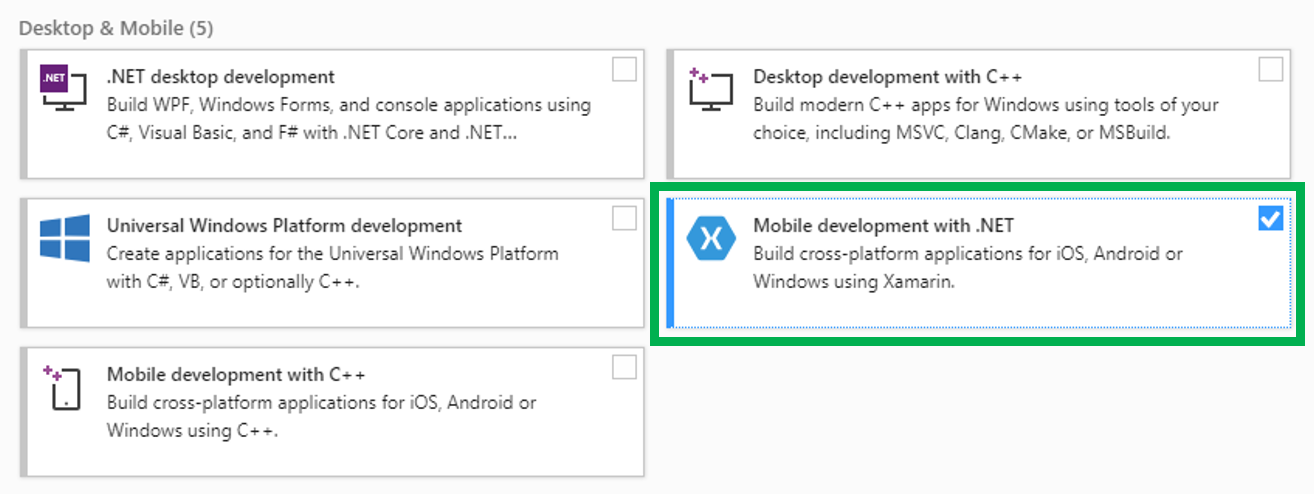
\includegraphics[width=0.9\linewidth]{images/auswahl_rahmenwerk/installation.png}    
    \caption{Auswahl des Xamarin-Rahmenwerks bei der Installation}
\end{figure}
Es empfiehlt sich, das Paket für \enquote{\acs{dotnet} desktop development} dazu zu installieren, damit neue, noch nicht bekannte \ac{dotnet}-Technologien in einer einfacheren Konsolen-Anwen\-dung ausprobiert werden können.
Das Paket benötigt ungefähr weitere 0.8GB.\par
Auf nähere Details der Installation von Visual Studio wird hier nicht eingegangen, diese können aber auf der Microsoft-Dokumentationsseite \cite[vgl.][]{msdoc-vs-install} nachgeschlagen werden.
%Betriebssystem, Hardwareanforderungen
%
\subsection{Android \acs{sdk}}
Um Xamarin-Applikationen für Android-Geräte entwickeln zu können wird das von Google bereitgestellte Android \ac{sdk} benötigt, um das Programm in ein \ac{apk} umzuwandeln. Die einzelnen Komponenten können im Android-\ac{sdk}-Manager des Visual Studio installiert werden.
Dieser ist im Menüband unter \enquote{Tools\textbackslash Android\textbackslash Android \ac{sdk} Manager} zu finden.
\begin{figure}[H]
    \centering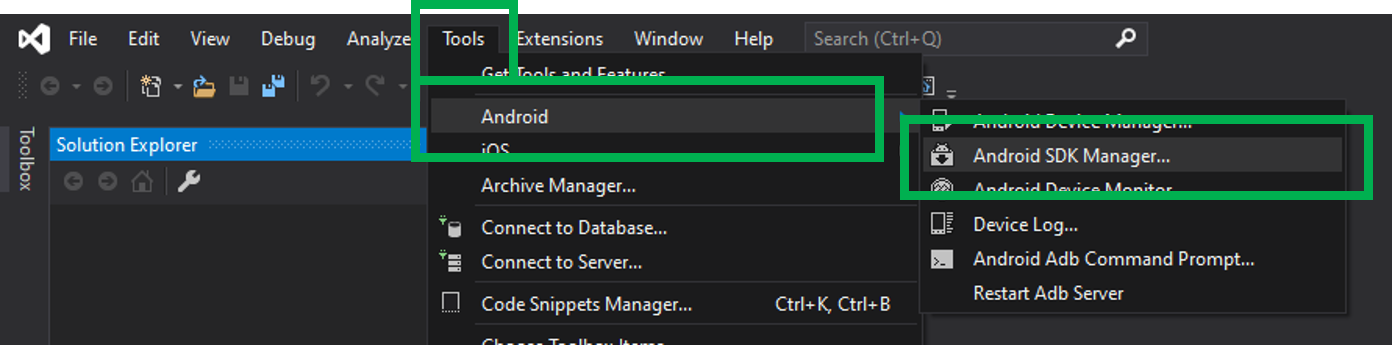
\includegraphics[width=0.9\linewidth]{images/auswahl_rahmenwerk/android_sdk_installation.png}    
    \caption{Android \acs{sdk} Manager}
\end{figure}
Der \ac{sdk}-Manager ist in zwei Seiten unterteilt - \enquote{Platforms} und \enquote{Tools}.\par

Auf der \enquote{Plat\-forms}-Seite können die benötigten \ac{sdk}-Teile für jede Android-Version installiert werden.
Benötigt wird nur die Version, mit der das Projekt später kompiliert werden soll.
Außerdem kann man auf dieser Seite des \ac{sdk}-Managers System-Abbilder für den Android Emulator installieren.\par

Über die \enquote{Tools}-Seite können verschiedenste Entwicklungswerkzeuge installiert werden.
Grundsätzlich erforderlich sind \enquote{Android \acs{sdk} Tools}, \enquote{Android \acs{sdk} Platform Tools} und \enquote{Android \acs{sdk} Build Tools} um Android-Apps mit Xamarin entwickeln zu können.
Für dieses Projekt werden Push-Benachrichtigungen via Google Cloud Messaging verwendet, daher werden noch zusätzlich die Pakete für die \enquote{Google Play Services} sowie die \enquote{Google Cloud Messaging for Android Library} installiert.
Wie Push-Benachrichtigungen genauer funktionieren wird später im Kapitel \crossref{ch:push} auf Seite \pageref{ch:push} behandelt.
\begin{figure}[H]
    \centering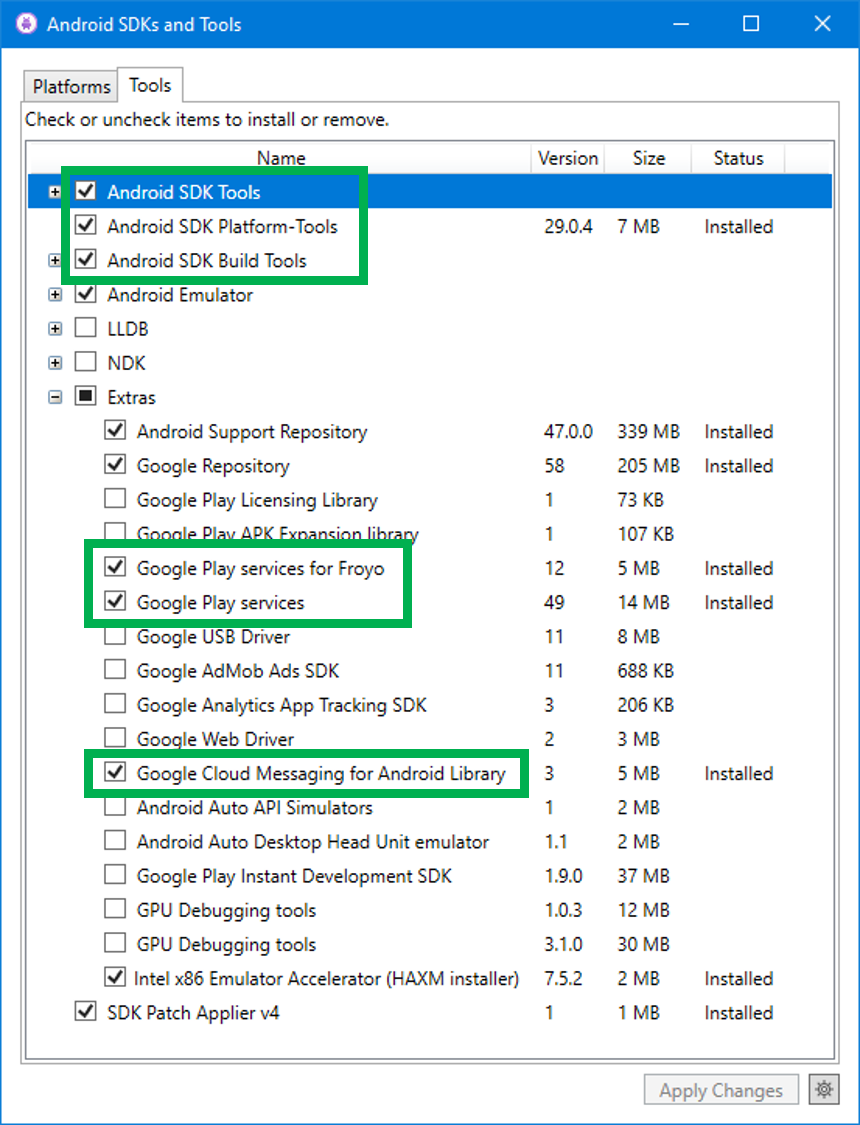
\includegraphics[width=0.8\linewidth]{images/auswahl_rahmenwerk/android_sdk_auswahl.png}    
    \caption{Notwendige Teile des Android \acs{sdk}}
\end{figure}

\subsection{Build-Vorgang}
Um den geschriebenen Code in eine lauffähige Applikation umzuwandeln wird ein sogenannter Compiler benötigt.
Die Aufgabe des Compilers ist es, die geschriebene Hochsprache entweder direkt in \acs{cpu}-Maschinensprache bzw. eine Art Zwischencode zu kompilieren, d.h. umzuwandeln. Im Fall einer einfachen C\#-Konsolenanwendung ist der Build-Vorgang noch relativ simpel:
\begin{enumerate}
    \item Alle einzelnen Code-Dateien werden nacheinander vom Compiler in \ac{cil}, eine Zwischensprache des \ac{dotnet}, umgewandelt.
    \item Der Linker fügt die einzelnen Teile zu einem Gesamten zusammen.
    Das Resultat ist eine Datei, die wie eine ausführbare .EXE-Datei erscheint.
    \item Wenn das zusammengefügte Programm gestartet wird, kompiliert die \ac{clr} den Zwischencode in ausführbaren Maschinen-Code.
    Die \acs{cpu} des Systems kann diesen dann ausführen.
\end{enumerate}
\begin{figure}[H]
    \centering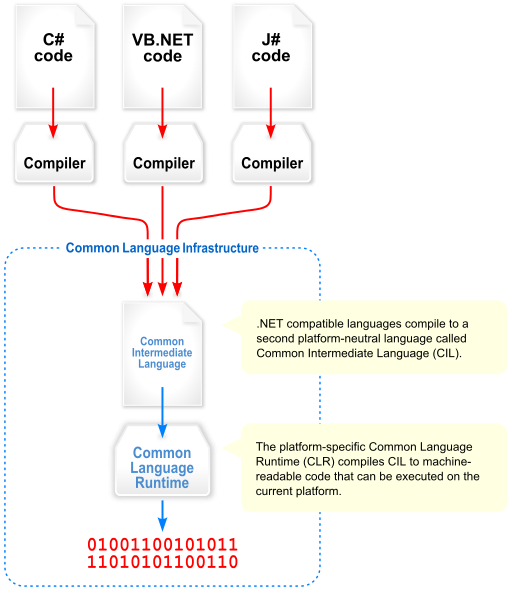
\includegraphics[height=12cm]{images/auswahl_rahmenwerk/dotnet-compilation.png}
    \caption{Build-Vorgang einer \ac{dotnet}-Applikation\cite{wiki-cli}}
    %\footfullcite[]{wiki-cli}
\end{figure}

Ähnlich funktioniert dieser Vorgang auch bei einer Xamarin.Forms-App, allerdings wesentlich komplexer.
Eine Xamarin.Forms-Solution besteht aus drei Einzel-Projekten (PiBell, PiBell.Android, PiBell.iOS), wobei das \acs{dotnet}-Standard-Projekt als Teil der anderen zwei verbaut werden muss.
Dadurch ergibt sich ein in Abbildung \crossref{fig:build-forms} dargestellter Build-Vorgang.
\begin{figure}
    \centering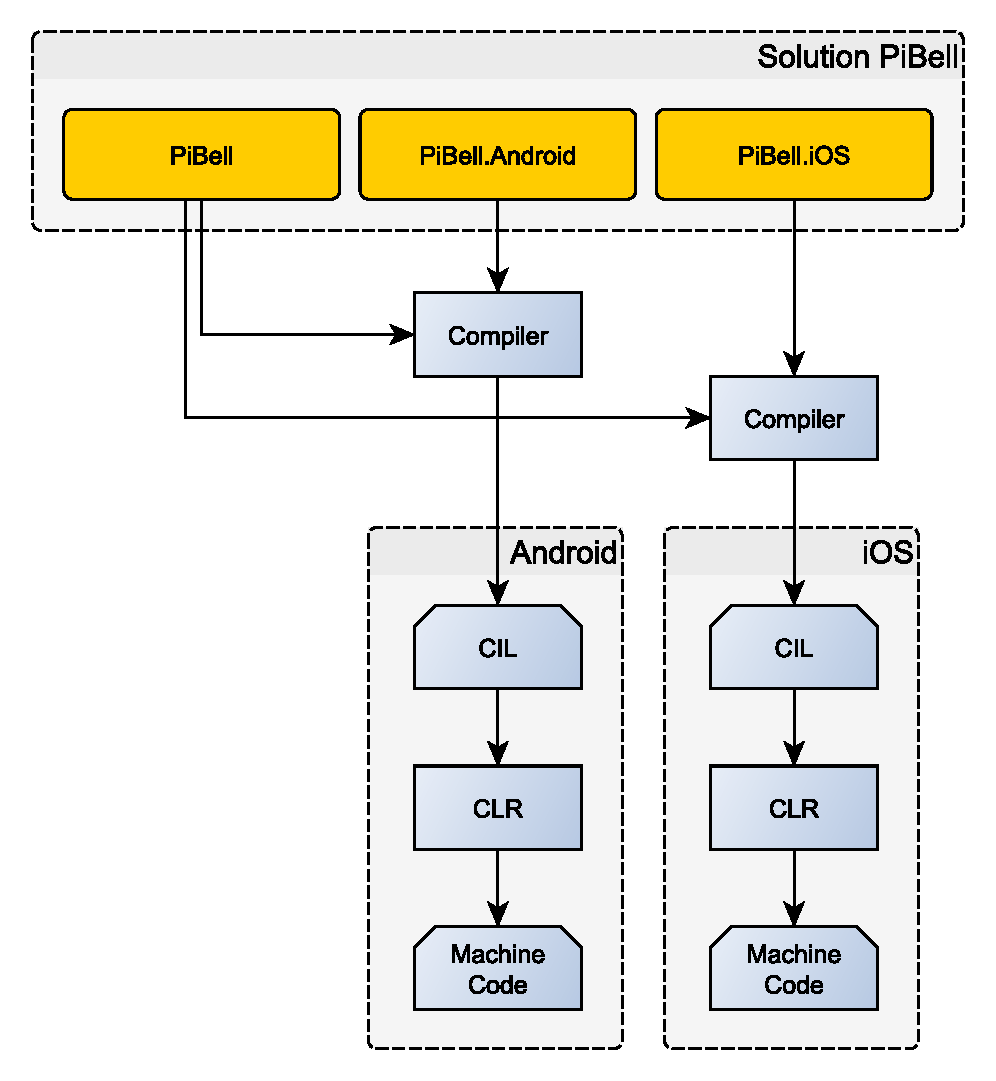
\includegraphics[width=0.9\linewidth]{images/auswahl_rahmenwerk/build-vorgang.pdf}
    \caption{Build-Vorgang einer Xamarin.Forms-Solution}
    \label{fig:build-forms}
\end{figure}

%Weg vom Programm zur binary
%microsoft VS2019
%frei zugänglich
%nur auf windows, kein linux-support
%...
\chapter{Verwendete Software-Module}
\section{\acl{rtsp}}
\acs{rtsp} ist ein Netzwerkprotokoll zum Aufbauen und Verwalten von Netzwerk-Verbindungen zur Übertragung kontinuierlicher Medien-Daten (Streams).
Dieses Netzwerkprotokoll ist im \acs{ietf}-Dokument \citetitle{ietf-rtsp} festgelegt. 
Es wurde gemeinsam von \citeauthor{ietf-rtsp} entwickelt. \cite[vgl.][]{ietf-rtsp}\par

\subsection{\acs{rtsp} Version 2}
Im Zuge dieser Diplomarbeit wird die erste Version des \acs{rtsp}-Protokolls verwendet.
Neben der verwendeten Version 1 existiert auch eine neue Version 2, welche im \acs{ietf}-Dokument \citetitle{ietf-rtsp-2} definiert ist. Die neue Version wurde von \citeauthor{ietf-rtsp-2} erarbeitet. \cite[vgl.][]{ietf-rtsp-2}
Es wurde dennoch die erste Version verwendet, da die Stationen dieses bereits verwenden und die neue Version nicht rückwärtskompatibel ist.\par

\acs{rtsp} wird in der Industrie vielseitig verwendet, um Live-Übertragungen von Überwachungskameras zu verwalten. Eine weitere Anwendung des \acs{rtsp} Protokolls ist das Streamen von Medien-Daten zu einem Server, der diese dann beispielsweise transcodiert oder aufnimmt.

\subsection{Anfragen-Aufbau}
Das \acs{rtsp}-Protokoll definiert mehrere Anfragen zur Verwaltung der Netzwerkverbindung.
Diese Anfragen werden, ähnlich wie beim \acs{http}, in unverschlüsseltem Plain-Text verschickt.
In Tabelle \ref{tab:rtsp-req} sind sämtliche Anfragen des \acs{rtsp}-Protokolls und deren Übertragungsrichtung aufgelistet.
Die in Tabelle \ref{tab:rtsp-req} verwendeten Kurzbezeichnungen haben folgende Bedeutung:
\paragraph{Richtung:} C\dots Client, S\dots Server
\paragraph{Objekt:}P\dots Präsentation, S\dots Stream
\begin{table}[H]
    \centering\begin{tabular}{|r|c|c|l|}
        \hline%-----------------------------------------------------------
        Methode         &Richtung                           &Objekt &Verbindlichkeit\\
        \hline%-----------------------------------------------------------
        DESCRIBE        &C$\rightarrow$S                    &P,S    &empfohlen\\
        ANNOUNCE        &C$\rightarrow$S, S$\rightarrow$C   &P,S    &optional\\
        GET\_PARAMETER  &C$\rightarrow$S, S$\rightarrow$C   &P,S    &optional\\
        OPTIONS         &C$\rightarrow$S, S$\rightarrow$C   &P,S    &erfordert, (S$\rightarrow$C: optional)\\
        PAUSE           &C$\rightarrow$S                    &P,S    &empfohlen\\
        PLAY            &C$\rightarrow$S                    &P,S    &erfordert\\
        RECORD          &C$\rightarrow$S                    &P,S    &optional\\
        REDIRECT        &S$\rightarrow$C                    &P,S    &optional\\
        SETUP           &C$\rightarrow$S                    &S      &erfordert\\
        SET\_PARAMETER  &C$\rightarrow$S, S$\rightarrow$C   &P,S    &optional\\
        TEARDOWN        &C$\rightarrow$S                    &P,S    &erfordert\\
        \hline%-----------------------------------------------------------
    \end{tabular}
    \caption{Anfrage-Arten des \acs{rtsp}-Protokolls}
    \label{tab:rtsp-req}
\end{table}
Das Aussehen einer solchen Anfrage wird anhand des Beispiels der DESCRIBE-Methode veranschaulicht.
Der Client beginnt die Anfrage mit dem \acs{url} des Medien-Streams, den er abrufen möchte und teilt dem Server mit, welche Formate er versteht.
\begin{lstlisting}
C->S: DESCRIBE rtsp://server.example.com/fizzle/foo RTSP/1.0
    CSeq: 312
    Accept: application/sdp, application/rtsl, application/mheg
\end{lstlisting}
Der Server antwortet auf diese Anfrage mit dem Session Descriptor, der alle wichtigen Informationen des Medien-Streams beinhaltet, wie zum Beispiel Video- und Audio-Format, Übertragungsmethode, sowie allgemeine Informationen wie Titel und Beschreibung.
\begin{lstlisting}
S->C: RTSP/1.0 200 OK
    CSeq: 312
    Date: 23 Jan 1997 15:35:06 GMT
    Content-Type: application/sdp
    Content-Length: 376

    v=0
    o=mhandley 2890844526 2890842807 IN IP4 126.16.64.4
    s=SDP Seminar
    i=A Seminar on the session description protocol
    u=http://www.cs.ucl.ac.uk/staff/M.Handley/sdp.03.ps
    e=mjh@isi.edu (Mark Handley)
    c=IN IP4 224.2.17.12/127
    t=2873397496 2873404696
    a=recvonly
    m=audio 3456 RTP/AVP 0
    m=video 2232 RTP/AVP 31
    m=whiteboard 32416 UDP WB
    a=orient:portrait
\end{lstlisting}

\section{LibVLC Sharp}
% LibVLC ist eine C-Bibliothek für die Medienverarbeitung und -Wiedergabe.
% Mit Hilfe von Bindings kann diese Bibliothek auch in anderen Programmiersprachen verwendet werden.
% Eines dieser Binding ist LibVLC Sharp, welches die Funktionen der LibVLC in C\# zur Verfügung stellt.
% Es handelt sich bei der LibVLC um ein OpenSource-Projekt der Organisation VideoLAN, das fortlaufend weiterentwickelt und unterstützt wird. Der sehr bekannte VLC Media Player nutzt für alle Funktionen die LibVLC und dient daher sozusagen als Grafische Oberfläche zur LibVLC. \cite[vgl.][]{libvlc}\par

% Im Zuge dieser Diplomarbeit wird das C\#-Binding der LibVLC verwendet, um am Smartphone den Video-Stream der fest installierten Station abrufen und darstellen zu können.
% Dies wird näher im Kapitel \crossref{ch:prog-doc} beschrieben.
LibVLC ist ein Multimedia-Rahmenwerk der Non-Profit-Organisation VideoLAN, welche durch den VLC Media Player und dessen Funktionsumfang bekannt wurde. Der VLC Media Player funktioniert sozusagen als grafische Oberfläche zur LibVLC-Programmbibliothek.
Die Bibliothek beinhält viele nützliche Funktionen, darunter die folgenden:
\begin{itemize}
    \item Videos nahezu beliebigen Formates decodieren und darstellen
    \item Video und Audio aufnehmen und Transcodieren für die weitere Verwendung
    \item Live-Streaming von Video-Daten, Webcam-Bild und Mikrofon-Ton.
\end{itemize}    
LibVLC ist eine Bibliothek für die C-Sprache. Um diese in einem C\#-Projekt verwenden zu können sind Bindings notwendig, welche Zugriff auf die C-Bibliothek geben.
LibVLC wurde von der Non-Profit-Organisation VideoLAN entwickelt und erstmals am 1. Februar 2001 veröffentlicht wurde.\cite{libvlc-release}\par

Im Xamarin.Forms-Projekt wird die zum Zeitpunkt der App-Entwicklung aktuelle Version 3.4.2 der LibVLC Sharp Bindings verwendet. Bindings erlauben es dem Programmierer auf Programmbibliotheken zuzugreifen, welche für eine andere Sprache geschrieben wurden. Man kann sich Bindings wie Kleber vorstellen, der die Funktionen der einen Programmiersprache mit denen der anderen Sprache verbindet. Die Version 3.4.2 ist inzwischen nicht mehr die neueste Version, jedoch  ist sie in Hinsicht auf Funktionalität deckungsgleich mit der neuesten Version.\par

\subsection{Erwähnenswerte Funktionen}
Die LibVLC-Sharp-Bindings ermöglichen die Verwendung des MVVM-Modells, welches vom WPF- und Silverlight-Architekten John Gossman im Jahr 2005 auf seinem Blog vorgestellt wurde. \cite[vlg.][The Evolution of Model-View-ViewModel]{msdoc-mvvm}
Die Philosophie hinter diesem Modell ist die Oberfläche (View) bis auf wenige Schnittstellen komplett vom eigentlichen Code zu trennen.
Dies ermöglicht es ohne größeren Aufwand die Oberfläche zu ändern oder gar auszutauschen.
Folgende Terminologie wird in diesem Zusammenhang verwendet:
\begin{itemize}
\item Models … beinhalten die Programmdaten. Meist sind einfache Klassen oder Strukturen hierfür verwendet.
\item Views … Die grafische Oberfläche und deren Elemente wie Buttons, TextBoxen, …
\item ViewModels … wandeln die Daten der Models so um, dass sie von der Oberfläche dargestellt werden können. ViewModels sind meist als Klasse ausgeführt.
\end{itemize}

Die Daten der Oberfläche und die Daten des Models bleiben zueinander konsistent. Sobald sich ein Wert auf einer Seite ändert, wird er sofort auf der anderen aktualisiert.
\begin{figure}[H]
    \centering
    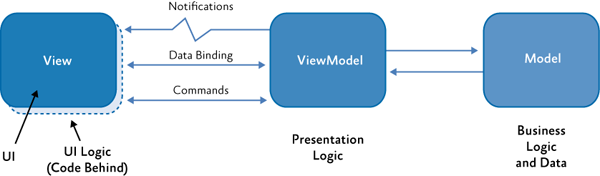
\includegraphics[width=.9\linewidth]{images/software_module/MVVM.png}
    \caption{Datenfluss MVVM}
\end{figure}
Das MVVM-Modell bietet sich auch an, wenn die Daten des Programms oft in eine andere Form gebracht werden müssen, bevor sie dargestellt werden können. Zum Beispiel wird vom Model die aktuelle Zeit als Ganzzahl abgespeichert, welche nur die vergangenen Millisekunden seit einem bestimmten Zeitpunkt zählt; um die Zeit allerdings darstellen zu können, muss diese Ganzzahl zuerst in ein lesbares Datumsformat gebracht werden. Diese Aufgabe würde das ViewModel übernehmen.

\subsection{Nachteile}
Sowohl die ursprüngliche LibVLC-Bibliothek, als auch die entsprechenden C\#-Bindings sind auf der offiziellen Dokumentationsseite nur spärlich dokumentiert.\cite[vgl.][]{libvlc-sharp-doc}
%quelle
Beispielsweise verwenden alle Beispielprojekte der LibVLC Sharp Bindings das MVVM-Modell, daher ist nicht bekannt, ob eine Implementierung ohne dieses Modell überhaupt möglich ist.
Weiters sind die einzelnen Funktionen zwar auf der Dokumentationsseite aufgelistet, allerdings nicht sehr ausführlich beschrieben. \cite[vgl.][]{libvlc-sharp-doc}

\subsection{Alternativen}
Während der Recherche wurden wenige Alternativen gefunden. Diese Alternativen sind jedoch seit langem nicht mehr in Entwicklung und sind daher nicht für die Verwendung empfohlen. Die LibVLC-Bibliothek ist momentan die einzige kostenfreie Variante \acs{rtsp}-Streams mit Xamarin auf dem Mobilgerät abspielen zu können. Es gibt Bibliotheken von VASTreaming, jedoch sind diese kostenpflichtig zu erwerben, was für diese Diplomarbeit keine Option ist. \cite[vgl.][Pricing]{vastreaming}

\section{GStreamer}
GStreamer ist ein extrem leistungsfähiges und vielseitiges Framework zur Erstellung von Medien-Streaming-Anwendungen.
Viele der Vorzüge des GStreamer-Frameworks liegen in seiner Modularität:
GStreamer kann neue Plugin-Module nahtlos integrieren.
Aber da Modularität und Leistungsfähigkeit oft mit einem Preis für eine größere Komplexität einhergehen, ist das Schreiben neuer Anwendungen nicht immer einfach.
\cite[aus dem Englischen übersetzt]{gstreamer}\par

GStreamer ist Pipeline-basiert, d.h. die Funktion wird mit einer Vielzahl von hintereinander geschalteten Filtern bestimmt.
Eine Pipeline hat immer einen Eingang (Source) und einen oder mehrere Ausgänge.
Zwischen diesen können sich beliebig viele Filter befinden, die unterschiedlichste Funktionen haben können:
\begin{itemize}
    \item Signale de- und encodieren (Codec, z.B. x264enc)
    \item Größe und Position von Videos verändern (Caps, z.B. video/x-raw)
    \item die Pipeline in zwei Teile auftrennen, z.B. in Video und Audio (Demux)
    \item Daten zu einem Netzwerk-Paket zusammenbündeln (z.B. rtph264pay)
    \item etc.
\end{itemize}
Ein Filter hat bestimmte Ein- und Ausgangsformate die er unterstützt.
Als Beispiel nehmen wir den H264-Encoder:
dieser unterstützt für das Eingangssignal RAW-Video, also decodierte Binärdaten. Am Ausgang kommt logischerweise ein H264-codierter Video-Stream heraus.\par

Das GStreamer-Rahmenwerk wird aktuell vom GStreamer-Team fortlaufend upgedatet und verbessert.
Die erste Version des GStreamer-Rahmenwerks wurde im Jahr 2001 mit der Versionsnummer 0.1.0 veröffentlicht.
Im Jahr 2012 kam eine große Umstellung, bei der grundlegende Teile des Rahmenwerks ausgetauscht wurden, wodurch einige Teile nicht mehr kompatibel waren.
Ab diesem Zeitpunkt begann die Versionsnummer mit 1.x.x, um die neuen Versionen deutlich von den Vorgängern abzutrennen.
Die aktuelle Version des GStreamer-Rahmenwerks zum Verfassungszeitpunkt dieser Arbeit ist die Version 1.16.2.\par

Aktuell wird die Version 1.16.2 verwendet. Da aber alle 1.x.x-Versionen mehr oder weniger miteinander kompatibel sind, kann sich das ändern, sobald ein neues Update veröffentlicht wird. Es gibt keinen besonderen Grund auf genau dieser Version zu bleiben.\par

Es wurden während der Recherche einige mögliche Alternativen für das GStreamer-Rahenwerk gefunden:
\begin{itemize}
    \item FFmpeg, ein Multimedia-Rahmenwerk, das vor allem im Bereich Transcodierung verwendung findet. Es bietet alle Funktionen des GStreamer-Rahmenwerks an.
    \item LibVLC, die Grundlage des VLC Media Players, welche vor allem zur Wiedergabe verwendet wird. Diese Bibliothek kann zur Transcodierung und Live-Übertragung genutzt werden, ist allerdings nicht dafür optimiert.
\end{itemize}

GStreamer wird in diesem Projekt verwendet, da bei Live-Video-Übertragung möglichst wenig Latenz vorkommen soll.
Das GStreamer-Rahmenwerk ist in dieser Hinsicht den anderen Multimedia-Rahmenwerken weit voraus.
Zusätzlich gibt es von GStreamer keine einschränkenden Vorgaben was Ein- und Ausgangsformat betrifft.
Es kann jede beliebige Quelle mit jedem beliebigen Output verknüpft werden, solange die richtige Pipeline verwendet wird.
Weiters ist das Projekt quelloffen, d.h. man ist in Bezug auf die Installationsdateien nicht auf den Hersteller angewiesen, sondern kann das Programm selbst für die jeweilige Plattform kompilieren, wenn der Hersteller das noch nicht getan hat.
Außerdem kann jeder Entwickler Vorschläge für Änderungen am Code, sowie Bugfixes vorbringen.
\subsection{Pipeline-Beispiel}
Die detaillierte Funktionsweise des GStreamer-Rahmenwerks lässt sich am besten anhand eines realistischen Beispiels erklären.
In diesem Beispiel wird ein in Echtzeit generiertes Testvideosignal zuerst auf 1280x720 Pixel vergrößert und danach als H264-encodierter Stream via RTP verschickt.
\begin{lstlisting}
    gst-launch-1.0 videotestsrc ! video/x-raw,width=1260,height=720,framerate=20/1 ! autovideoconvert ! queue ! x264enc tune=zerolatency bitrate=4096 speed-preset=superfast ! queue ! rtph264pay config-interval=1 mtu=1300 ! udpsink host=127.0.0.1 port=5000
\end{lstlisting}
Der Filter \enquote{queue} wird hier verwendet, um vor und nach dem Encoding-Vorgang ein kurzes Video-Segment in einem Zwischenspeicher zu behalten. Dies ist notwendig, da der H264-Codec mehrere Video-Frames auf einmal komprimiert.

\subsection{gst-rtsp-server}
gst-rtsp-server ist ein Zusatzmodul für das GStreamer- Rahmenwerk, welches die Verwendung des \acs{rtsp}-Protokolls 

\section{Live555 Proxy}
Ein \acs{rtsp}-Stream ist grundsätzlicherweise eine Unicast-Verbindung zwischen Server und Client.
Falls mehrere Clients den gleichen Medien-Stream abrufen möchten, muss der Server diesen für jeden Client einzeln transcodieren und verschicken.
Dies stellt eine große Belastung für den Server un dessen Internetanbindung dar.
Mit Hilfe eines Proxy-Servers muss der Medien-Stream nur einmal verarbeitet werden, bevor er dann an die einzelnen Clients verteilt wird.\par

Der Live555 Proxy Server ist eine quelloffene Applikation, welche für genau diese Aufgabe von LiveMedia Inc. entwickelt wurde.
Mit Hilfe des Live555 Proxy Servers wird ein \acs{rtsp}-Stream einmalig eingelesen und an alle verbundenen Clients verteilt.
Dadurch bleibt die \acs{cpu}-Belastung des Servers unabhängig von der Anzahl der verbundenen Clients, wodurch er unter Umständen mehrere verschiedene Streams bereitstellen könnte. Für jeden Medien-Stream, den der Server anbietet, wird eine weitere Live555-Proxy-Server-Instanz benötigt.\par

Der Live555 Proxy Server wurde im Jahr xxxx erstmals von LiveMedia Inc. veröffentlicht. Neben dem Live555 Proxy Server entwickelt das Unternehmen mehrere Projekte:
\begin{itemize}
    \item Live555 Media Server, mit dem lokale Medien-Dateien per \acs{rtsp} dem Netzwerk bereitgestellt werden können.
    \item liveCaster, zur Multicast-Übertragung von MP3-Dateien
    \item diverse Kommandozeilenprogramme zum Senden und empfangen von Echtzeit-Streams
\end{itemize}
Die von LiveMedia Inc. entwickelten Programme und Bibliotheken finden in vielen bekannten Applikationen Anwendung, darunter auch der VLC Media Player mit der dazugehörigen LibVLC. In diesem Programm werden die Live555-Bibliotheken zum Empfangen und Entschlüsseln von \acs{rtsp}-Streams genutzt.
\chapter{Push-Benachrichtigung}
\label{ch:push}
\section{Push Notification Service}
Eine Notification dient dazu den Benutzer über etwas zu informieren. Dies kann ein Kalender-Eintrag, eine eingetroffene \ac{sms} oder ein anderes Ereignis sein. Diese Art der Benachrichtigung wird meist über eine Local Notification erzeugt. Eine Local Notification wird aufgrund eines lokal am Gerät auftretenden Ereignisses ausgelöst. Eni Beispiel ist in Abbildung \ref{fig:local-notification} zu sehen.
\begin{figure}
    \centering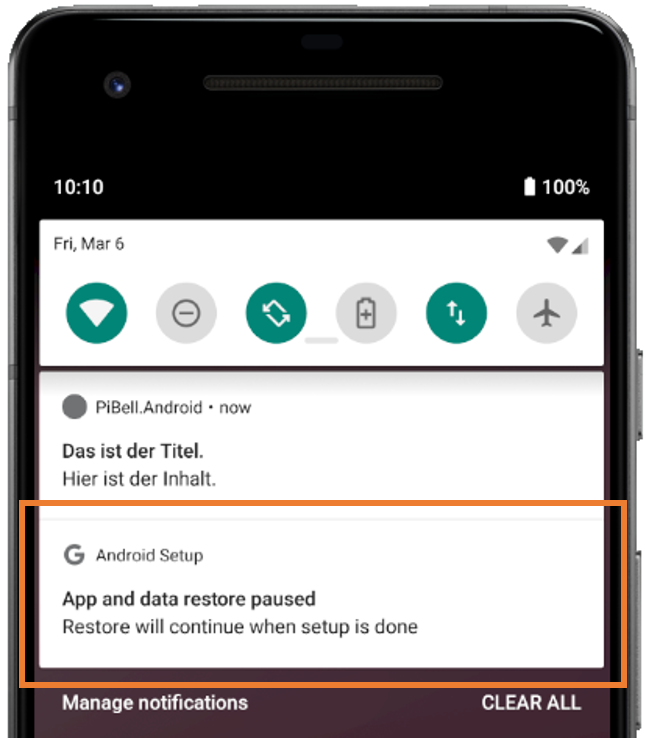
\includegraphics[width=.5\linewidth]{images/xamarin/LocalNotification.png}
    \caption{Lokale Benachrichtigung}
    \label{fig:local-notification}
\end{figure}

Im Gegensatz dazu dient eine Push Notification dazu, ein externes Ereignis auf einem anderen Gerät zu verarbeiten.
Das Empfängergerät zeigt in den meisten Fällen eine zusätzliche Local Notification dem Benutzer an.
Beispiele für Push Notifications sind Katastrophenwarnungen, neue Instant-Messenger-Nachrichten, oder ähnliche Ereignisse, die nicht auf dem Empfängegerät ihren Ursprung haben.

\subsection{Funktionsweise}
Eine Push Notification wird immer von einem sogenannten Push Notification Service an alle Zielgeräte geschickt.
Dieser Service wird vom jeweiligen Betriebssystem-Hersteller bereitgestellt.
Im Fall der hier entwickelten App sind das Google und Apple, mit ihren Push Notification Services \ac{gcm} und \ac{apns}.\par

Der Service ist dafür verantwortlich, die Benachrichtigung an alle registrierten Zielgeräte zu schicken.
Wenn das Zustellen nicht möglich ist, bricht der Service die Zustellung nach mehreren Versuchen für dieses Gerät ab.
Alle anderen Geräte erhalten die Benachrichtigung.
Daher ist es nicht sichergestellt, dass eine Push-Benachrichtigung bei jedem Gerät ankommt.\par

Zusätzlich zum Nachrichtentext können bei einer Push Notification zusätzliche Daten mitgeschickt werden. Diese können zum Beispiel die App über die genaue Benachrichtigungsursache informieren.

\section{AppCenter Push}
AppCenter Push hat in erster Linie die Funktion, den Zugriff auf die verschiedenen Push Notification Services zu vereinheitlichen und damit einfacher zu gestalten.
Microsoft AppCenter verwaltet alle Server-\ac{api}-Schlüssel, Zielgerätelisten und ähnliche Einstellungen, um den Prozess des Benachrichtigung-Sendens zu vereinfachen.
AppCenter Push ist entweder über das Web-Interface unter \url{https://appcenter.ms/} oder über die AppCenter \ac{api} erreichbar und verwendbar.\par

Die AppCenter Push \ac{sdk} abstrahiert den ganzen Prozess der Geräte-Registration, des Registrieren des Eingangs-Events und versteckt alles hinter einer einzelnen simplen Funktion \texttt{AppCenter.Start(„{App Secret}“, typeof(Push));}. Das App Secret ist der von AppCenter zugewiesene Schlüssel mit dem sichergestellt wird, dass das Gerät für das richtige AppCenter Projekt registriert wird.
Ohne diese \ac{sdk} müsste in der App viel mehr konfiguriert werden, was einen höheren Programmieraufwand und größere Fehlerrate darstellt. Außerdem würde das Rad neu erfunden werden.\par

In der entwickelten App wird die AppCenter-\ac{sdk}-Version 2.6.4 verwendet. Zu beachten ist, dass AppCenter Push nicht mehr weiterentwickelt und irgendwann dieses Jahr der Service abgeschaltet wird, wie es John Wargo in seinem Blog-Post am 3. Februar 2020 schrieb. Als Alternative wird von Microsoft der Azure-Notification-Hubs-Dienst angeboten. Bevor AppCenter Push endgültig terminiert wird, will Microsoft detaillierte Anleitungen zum Umstieg auf Azure bereitstellen.
\chapter{Programm-Dokumentation}
% Im Juni 2000 stellte das Unternehmen Microsoft das \ac{dotnet} vor.
% Kurz darauf wurde von Miguel de Icaza das sogenannte Mono-Projekt als Open-Source gestartet, welches eine Linux-Version des \ac{dotnet} darstellen soll.
% Am 16. Mai 2011 kündigt Miguel de Icaza an, dass das Mono-Projekt vom Unternehmen Xamarin weiterentwickelt wird, wobei einige wichtige Mitglieder des Mono-Entwickler-Teams weiterhin daran beteiligt sind.

% Das Unternehmen Xamarin wurde mit der Absicht gegründet, Software auf mobile Geräte zu vertreiben. 
\label{ch:prog-doc}
\section{Übersicht}
Das im Zuge dieser Diplomarbeit entwickelte Software-Projekt basiert auf einer der von Microsoft bereitgestellten Xamarin.Forms-Vorlagen, welche als Teil von Visual Studio bereitgestellt werden.
Es gibt mehrere Auswahlmöglichkeiten, wobei alle Vorlagen bis auf \enquote{Blank} Beispielcode beinhalten.
Da der Beispielcode der anderen Vorlagen für dieses Projekt nicht relevant ist und ohnehin gelöscht werden müsste, wird die \enquote{Blank}-Vorlage verwendet.
Diese Vorlage beinhält nur eine Haupt-Oberflächenseite ohne jeglichen Beispielcode.

Der immer wieder vorkommende Name PiBell ist eine freigeistliche Erfindung. PiBell ist der Projektname, der sich aus \acl{rpi} und \enquote{Bell}, dem englischen Wort für Klingel oder Glocke, zusammensetzt.

Visual Studio organisiert alle Programmteile in einer sogenannten Solution, welche den Projektnamen trägt. In diesem Fall beinhält die Solution \enquote{PiBell} drei Programmteile oder \enquote{Projects}:
\paragraph{PiBell} ist das portable Projekt, auch .NET-Standard-Projekt genannt.
Dieses beinhaltet den ganzen plattformunabhängigen Code, sowie die Definition der UI-Oberfläche mittels XAML-Dateien.
In diesem Projekt befindet sich der größte entwickelte Code-Anteil, da die meisten Funktionen, wie das Abspielen von Videos mit Hilfe der LibVLC-Bindings, plattformunabhängig funktionieren und deswegen geteilt werden können.

\paragraph{PiBell.Android} beinhaltet allen Code, der plattformspezifisch für Android geschrieben wurde.
Unter anderem ist hier enthalten die Android-Implementation des Mikrofon-Auf\-nahme-Services, sowie das Berechtigungs-Management.
Die Mikrofon-Aufnahme erfolgt auf einer sehr hardwarenahen Ebene, was die plattformabhängigkeit erklärt.

\paragraph{PiBell.iOS} beinhaltet wie PiBell.Android den plattformspezifischen Code für die iOS-Platt\-form. Aufgrund mangelnder Entwicklungswerkzeuge wurde dieser Teil nicht großartig behandelt.\par

\begin{figure}[H]
\centering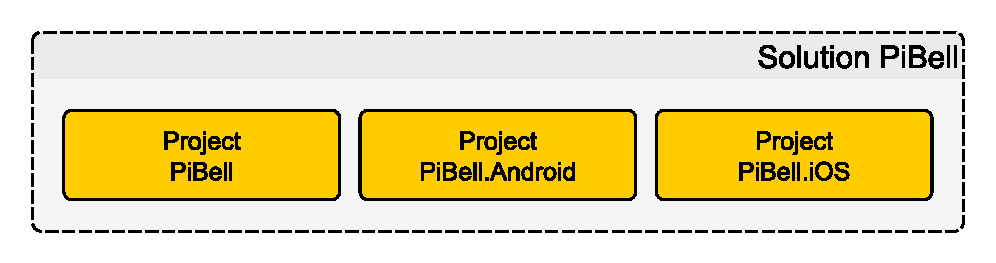
\includegraphics[width=0.9\linewidth]{images/xamarin/struktur.pdf}
\caption{Aufbau der Solution}
\end{figure}

%besteht aus drei teilen
%- portable project/.net standard project
%   plattformunabhängiger teil, oberfläche, ...
%- Android project
    %android-spezifischer teil, berechtigungen, ...
%- iOS project
    %iOS-spezifischer Teil, ...
%project-name PiBell -> erfindung, leitet sich aus raspberry und Türglocke ab
%
\section{Portable Project}
\section{PiBell.Android}
\section{PiBell.iOS}
\chapter{Testen}
\chapter{Ausblick}
\section{Gesicherte Verbindung}% VPN-Zugriff
\cleartoverso

\renewcommand{\authorName}{\AndreasGrain / \MatthiasMair}
\appendix
%\printbibheading
%\printbibliography[heading=subbibliography,type=online,title={Online-Quellen}]
%\printbibliography[heading=subbibliography,nottype=online,title={Andere Quellen}]
\printbibliography\clearpage
\printacronyms[heading=chapter*,name=Abkürzungen]\clearpage
\listoffigures\clearpage
\listoftables\clearpage

\part{Appendix}
\chapter{Verwendete Entwicklungswerkzeuge}
\chapter{Datenblätter}
\chapter{Kostenübersicht}
\chapter{Fertigungsdokumentation}
\end{document}